
\section*[Basics]{The very, very, basics of programming with Python}
\begin{frame}[plain]
\textbf{The very, very, basics of programming}\\
\vspace{1cm}
See also Chapter 4.
\end{frame}
\subsection*{Datatypes}


\begin{frame}{Python lingo}
\begin{block}{Basic datatypes (variables)}
\begin{description}
\item[{\color{red}int}] \texttt{32}
\item[{\color{red}float}] \texttt{1.75}
\item[{\color{red}bool}] \texttt{True}, \texttt{False}
\item[{\color{red}string}] \texttt{"Damian"}
\onslide<2->{\scriptsize \item[({\color{red}variable name}] \texttt{firstname})}
\end{description}
\end{block}
\onslide<2->{\textbf{"firstname" and firstname is not the same.\\}}
\onslide<3->{\textbf{"5" and 5 is not the same.}\\ But you can transform it: {\tt{int("5")}} will return 5.}\\
\onslide<3->{\textbf{You cannot calculate \texttt{3 * "5"}} {\tiny{(In fact, you can. It's \tt{"555"})}}.\\
But you can calculate {\tt{3 * int("5")}}}
\end{frame}



\begin{frame}{Python lingo}
\begin{block}{More advanced datatypes}
\begin{description}
\item[{\color{red}list}]<2-> \texttt{firstnames = $[$'Damian','Lori','Bjoern'$]$ \\ lastnames = $[$'Trilling','Meester','Burscher'$]$}
\item[{\color{red}list}]<3->\texttt{ages = $[$18,22,45,23$]$}
\item[{\color{red}dict}]<4-> \texttt{familynames= \{'Bjoern': 'Burscher', 'Damian': 'Trilling', 'Lori': 'Meester'\} }
\item[{\color{red}dict}]<4-> \texttt{\{'Bjoern': 26, 'Damian': 31, 'Lori': 25\} }

\end{description}
\pause
Note that the elements of a list, the keys of a dict, and the values of a dict can have any datatype! (Better to be consistent, though!)
\end{block}
\end{frame}


\subsection*{Functions and methods}
\begin{frame}{Python lingo}
\begin{block}{Functions}
\begin{description}
\item[{\color{red}functions}]<2-> Take an input and return something else \\ {\tt{int(32.43})} returns the integer 32. \texttt{len("Hello")} returns the integer 5.\\ 
\item[{\color{red}methods}]<3-> are similar to functions, but directly associated with an object. {\tt{"SCREAM".lower()}} returns the string "scream"
\end{description}
\end{block}
\onslide<4->{Both functions and methods end with \texttt{()}. Between the \texttt{()}, \emph{arguments} can (sometimes have to) be supplied.}
\end{frame}


\begin{frame}[fragile]{Writing own functions}
You can write an own function:
\begin{lstlisting}
def addone(x):
    y = x + 1
    return y
\end{lstlisting}

Functions take some input (``argument'') (in this example, we called it \texttt{x}) and \emph{return} some result.
	
Thus, running
\begin{lstlisting}	
addone(5)
\end{lstlisting}
returns \tt{6}.
\end{frame}



\subsection*{Modifying lists and dictionaries}

\begin{frame}[plain]
Modifying lists and dictionaries
\end{frame}{}
	
\begin{frame}[fragile]{Modifying lists}
\begin{block}{Appending to a list}
\begin{lstlisting}
mijnlijst = ["element 1", "element 2"]
anotherone = "element 3"   # note that this is a string, not a list!
mijnlijst.append(anotherone)
print(mijnlijst)
\end{lstlisting}
gives you:
\begin{lstlisting}
["element 1", "element 2", "element 3"]
\end{lstlisting}
\end{block}
\end{frame}



\begin{frame}[fragile]{Modifying lists}
\begin{block}{Merging two lists (= extending)}
\begin{lstlisting}
mijnlijst = ["element 1", "element 2"]
anotherone = ["element 3", "element 4"]
mijnlist.extend(anotherone)
print(mijnlijst)
\end{lstlisting}
gives you:
\begin{lstlisting}
["element 1", "element 2", "element 3", "element 4]
\end{lstlisting}
\end{block}
\end{frame}




\begin{frame}[fragile]{Modifying dicts}
\begin{block}{Adding a key to a dict (or changing the value of an existing key)}
\begin{lstlisting}
mydict = {"whatever": 42, "something": 11}
mydict["somethingelse"] = 76
print(mydict)
\end{lstlisting}
gives you:
\begin{lstlisting}
{'whatever': 42, 'somethingelse': 76, 'something': 11}
\end{lstlisting}
If a key already exists, its value is simply replaced.
\end{block}
\end{frame}




\subsection*[Indention]{Indention: The Python way of structuring your program}
\begin{frame}[plain]
Indention: The Python way of structuring your program
\end{frame}


\begin{frame}[fragile]{Indention}
\begin{block}{Structure}
The program is structured by TABs or SPACEs
\end{block}

\end{frame}



{\setbeamercolor{background canvas}{bg=black}
\begin{frame}[plain]
\makebox[\linewidth]{
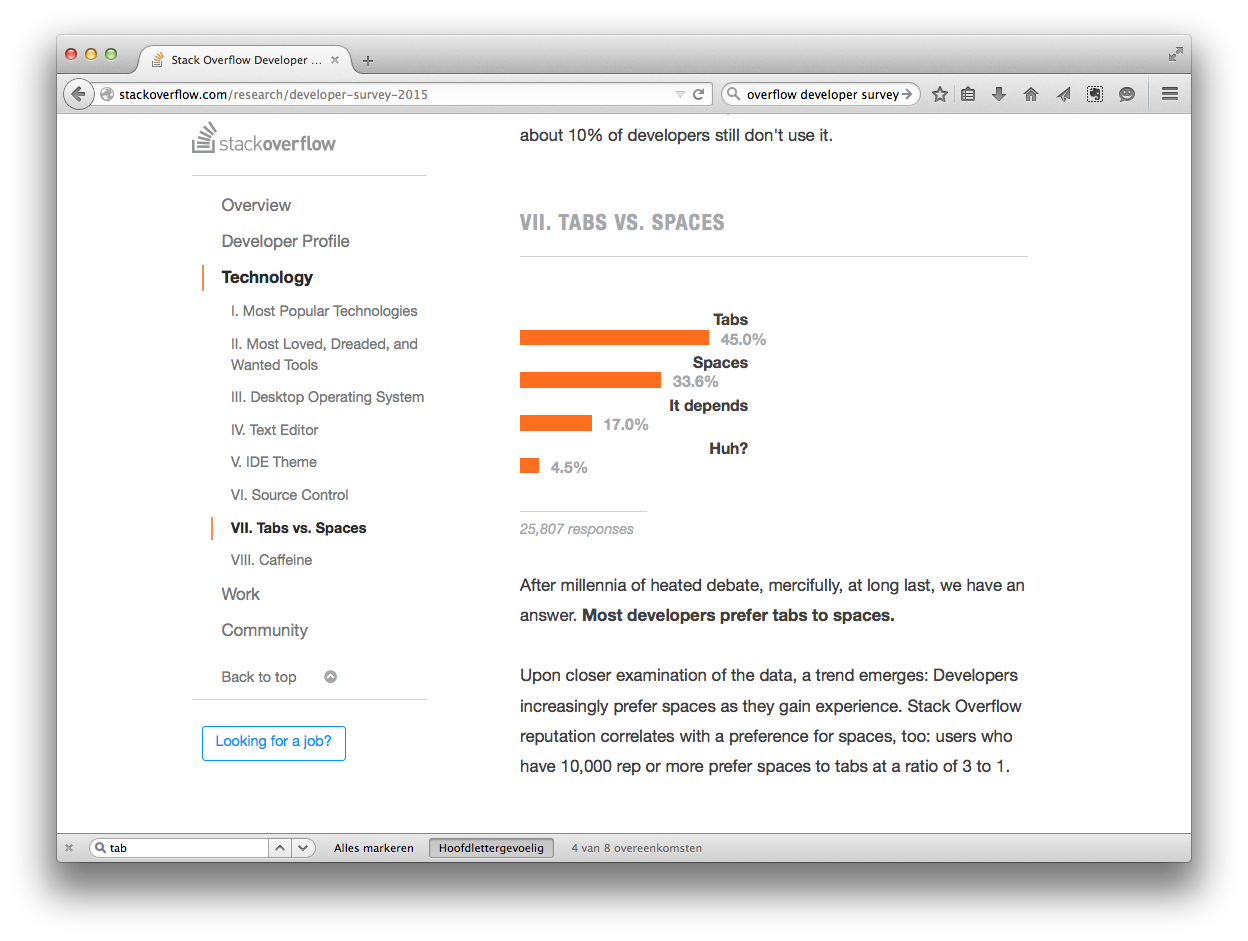
\includegraphics[width=\paperwidth,height=\paperheight,keepaspectratio]{../pictures/tabsvsspaces}
}
\end{frame}
}

\begin{frame}[fragile]{Indention}
\begin{block}{Structure}
The program is structured by TABs or SPACEs
\end{block}
\begin{lstlisting}
firstnames=['Damian','Lori','Bjoern']
age={'Bjoern': 27, 'Damian': 32, 'Lori': 26}
print ("The names and ages of these people:")
for naam in firstnames:
    print (naam,age[naam])
\end{lstlisting}
\onslide<2->{\textbf{Don't mix up TABs and spaces! Both are valid, but you have to be consequent!!! Best: always use 4 spaces!}}
\end{frame}





\begin{frame}[fragile]{Indention}
\begin{block}{Structure}
The program is structured by TABs or SPACEs
\end{block}
\begin{lstlisting}
print ("The names and ages of all these people:")
for naam in firstnames:
    print (naam,age[naam])
    if naam=="Damian":
        print ("He teaches this course")
    elif naam=="Lori":
        print ("She is a former assistant")
    elif naam=="Bjoern":
        print ("He helped teaching this course in the past")
    else:
        print ("No idea who this is")
\end{lstlisting}
\end{frame}


\begin{frame}{Indention}
The line \emph{before} an indented block starts with a \emph{statement} indicating what should be done with the block and ends with a \texttt{:}

\begin{block}{Indention of the block indicates that}<2->
\begin{itemize}
\item<3-> it is to be executed repeatedly (\texttt{for} statement) – e.g., for each element from a list
\item<4-> it is only to be executed under specific conditions (\texttt{if}, \texttt{elif}, and \texttt{else} statements)
\item<5-> an alternative block should be executed if an error occurs (\texttt{try} and \texttt{except} statements)
\item<6-> a file is opened, but should be closed again after the block has been executed (\texttt{with} statement)
\end{itemize}
\end{block}
\end{frame}


\section*{Exercise}
\subsection**{Exercise}
\begin{frame}
We'll now together do some simple exercises \ldots
\end{frame}



\begin{frame}{Exercises}
\begin{block}{1. Warming up}
\begin{itemize}
	\item Create a list, loop over the list, and do something with each value (you're free to choose). 
\end{itemize}
\end{block}
\begin{block}{2. Did you pass?}
	\begin{itemize}
	\item Think of a way to determine for a list of  grades whether they are a pass (>5.5) or fail.
	\item Can you make that program robust enough to handle invalid input (e.g., a grade as 'ewghjieh')?
	\item How does your program deal with impossible grades (e.g., 12 or -3)?
	\item \ldots
\end{itemize}
\end{block}
\end{frame}